%!TEX root = P231_notes.tex
\section{Coupled Harmonic Oscillators and Fields}
\label{sec:CHO:fields}

Let's take a break from Green's functions. In the previous section, we called the wave equation the \emph{harmonic oscillator in spacetime}. We proceeded to solve the wave equation for the electromagnetic field, $\partial^2 A_\mu = j_\mu$. We were very hand-wavy in arguing that the appropriate generalization of the harmonic oscillator operator $(d/dt)^2$ is the spacetime second derivative, $\partial^2 = c^{-2}\partial_t^2 - \nabla^2$. Furthermore, we noticed that our state functions went from being functions of only one variable, $\psi(t)$, to functions of space and time, $A_\mu(\vec{x},t)$. In other words, our states became \emph{fields}. It's instructive to see why a field is naturally understood as the continuum limit of a lattice of harmonic oscillators\footnote{I'm saying something `deep' here. Actual systems in condensed matter physics are atomic lattices with complicated electronic potentials. These are approximated by harmonic oscillators to leading order. At long wavelengths, the physics of this lattice often has a \emph{continuum limit} described by a field theory. The field theory is a model that has no underlying lattice, but whose long-wavelength predictions are designed to match that of a lattice with small spacing. In particle physics one usually assumes that nature is continuous so that the fundamental objects are actually fields. Whether or not this is literally true doesn't matter: it is sufficient that the range of phenomena that your theory hopes to describe are agnostic to whether or not there is a lattice. Sometimes particle physicists go the opposite way and use lattice techniques to make predictions where the continuum limit is difficult. The notion (and meaning) of a continuum limit is tied closely to the idea or renormalization group flow, which is one of the most elegant ideas in theoretical physics.}.


\subsection{A notational interlude}

Here's a bad habit: I often use the shorthand $x(t)$ to describe the position of a particle at time $t$. The particle doesn't need to literally be a particle, it could be the displacement of a spring from equilibrium. If the particle takes a position in three-space then we write $\vec{x}(t)$. Note that this is very different from a \emph{field}, where the spatial coordinates are a \emph{dependent} variable analogous to time. Just as $x(t)$ has a value for all $t$, a field $\varphi(x,t)$ takes some value for all $x$ and $t$. 

This is a potential source of confusion because we want to show the transition from a single harmonic oscillator to a field. The intermediate state is a lattice of coupled harmonic oscillators. To do this, let us break the bad habit of writing $x(t)$ and write the displacement of a harmonic oscillator to be $q(t)$. The displacement can be abstract, it doesn't have to be a distance separation; for example, it could be the value of a wavefunction at a point in space. If we have a bunch of harmonic oscillators evenly spaced on a line, we can index them $q_i(t)$. 

If you imagine that you have \emph{many} harmonic oscillators that are spaced very closely together, then rather then specifying an index you could just specify their position along the line, $x$. Note that $x$ is playing the role of an index, not as the state variable. In other words:
\begin{align}
	q_i(t) \to q(x,t) \ .
\end{align}
If I pick some point along the line, $x$, then the displacement of the harmonic oscillator at $x$ observed at time $t$ is $q(x,t)$. Congrats, $q(x,t)$ is now a field. You can see why we didn't want to use $x(t)$: it confuses the position along the line with the displacement of the harmonic oscillator at that position. 
%
The picture is as follows:
\begin{center}
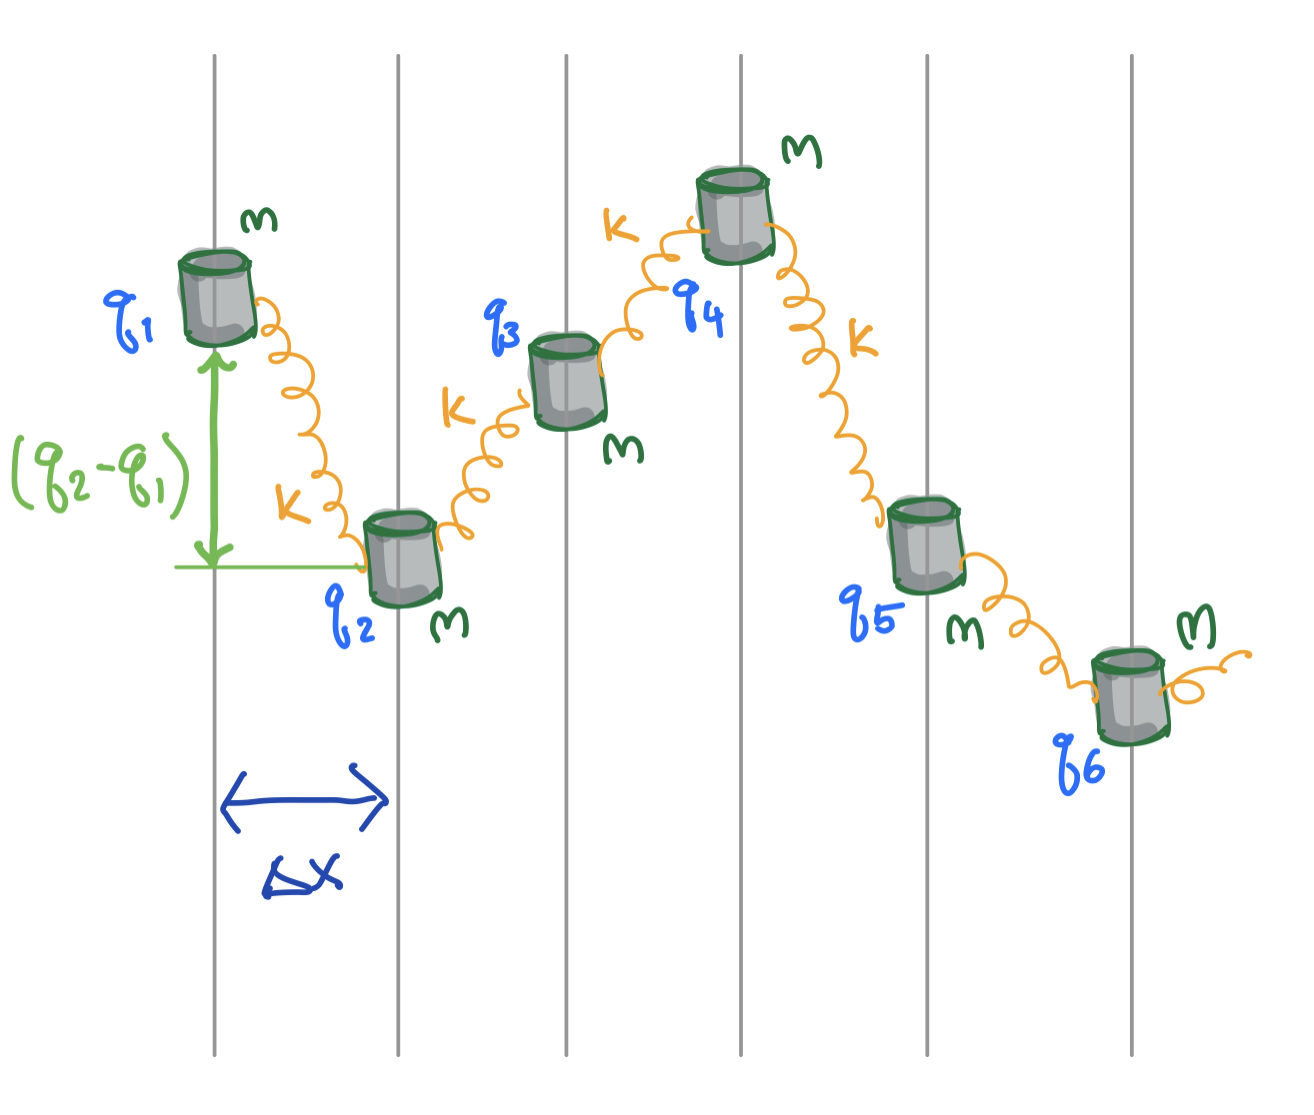
\includegraphics[width=.5\textwidth]{figures/coupledHO.jpg}
\end{center}
The generalization to a dense three-dimensional lattice is straightforward, you end up with $q(x,y,z,t)$ or $q(\vec{x},t)$.


\subsection{Coupled Harmonic Oscillators}
\label{sec:CHO}

The Lagrangian for a single harmonic oscillator $q(t)$ is
\begin{align}
	L[q(t)] &= \frac{1}{2}m \dot q^2 - \frac{1}{2}k q^2 \ .
\end{align}
This assumes some reference equilibrium value $q=0$. Consider instead a series of identical beads of mass $m$ along a line that can move up and down freely, but are connected to their nearest neighbors by springs of uniform spring constant $k$. The Lagrangian for this system is
\begin{align}
	L[q_1(t), q_2(t), \cdots]
	&= 
	\sum_i \frac{1}{2} m \dot q_i^2 
	- 
	\sum_i \frac{1}{2}k (q_i - q_{i-1})^2 \ .
\end{align}
Because life is short, I'm not going to worry about the boundary conditions for the index $i$. You can assume that the system is periodic if you're nervous. Now let us pass into the continuum limit and consider some small separation $\Delta x$. We make the following replacement to continuum variables:
\begin{align}
	i & \rightarrow x
	\\
	q_i(t) & \rightarrow q(x,t)
	\\
	(q_i-q_{i-1})^2 &\rightarrow \Delta x^2 \left(\frac{\partial q}{\partial x}\right)^2
	\\
	\sum_i	&\rightarrow \int \frac{dx}{\Delta x}
	\\
	m &\rightarrow \rho \Delta x \ .
\end{align}
The factors of $\Delta x$ should be clear from dimensional analysis. You can think about them as some characteristic small length scale analogous to the lattice spacing. Observe that the mass of a single harmonic oscillator is replaced by the mass density $\rho$ multiplied by a `volume' ($\Delta x$ in one dimension). Once we write out the Lagrangian the $\Delta x$ factors almost cancel:
\begin{align}
	L 
	&= \int \frac{dx}{\Delta x} \, 
	\left[
		\frac{1}{2}\rho \Delta x 
		\left(\frac{\partial q}{\partial t}\right)^2 
		- 
		\frac{1}{2}k \Delta x^2
		\left(\frac{\partial q}{\partial x}\right)^2
	\right]
	\\
	&= \int dx\,
	\left[
		\frac{1}{2}\rho 
		\left(\frac{\partial q}{\partial t}\right)^2 
		- 
		\frac{1}{2} \left(k \Delta x\right)
		\left(\frac{\partial q}{\partial x}\right)^2
	\right] \ .
\end{align}
If we had a lattice in $D$ spatial dimensions, then this result generalizes to
\begin{align}
	L 
	&= \int d^Dx\,
	\left[
		\frac{1}{2}\rho 
		\left( \frac{\partial q}{\partial t} \right)^2 
		- 
		\frac{1}{2} \left(k \Delta x^{2-D}\right)
		\left(\frac{\partial q}{\partial \vec{x}}\right)^2
	\right] \ .
	\label{eq:HO:coupled:D}
\end{align}
Finally, let us rescale the state variable by defining a `better' state variable
\begin{align}
	\varphi(x,t) \equiv \frac{q(x,t)}{\sqrt{\rho}} \ .
	\label{eq:field:normalization}
\end{align}
Further, let's go ahead and write the action $S=\int dt \, L$ with the idea of writing one big \emph{spacetime} integral over a Lagrangian \emph{denstiy} $S = \int dt\, d^Dx \, \mathcal L$:
\begin{align}
	S = \int dt \, d^Dx \,
	\frac{1}{2}
	\left[
	\left( 
		\frac{\partial \varphi}{\partial t}
		\right)^2
	- 
	c^2
	\left(\frac{\partial \varphi}{\partial \vec{x} }\right)^2
	\right] \ .
\end{align}
Observe that we have defined a speed
\begin{align}
	c^2 = k \Delta x^{2-D} \rho \ .
	\label{eq:HO:coupled:D:c2}
\end{align}
If we take one more step and integrate by parts, we may write the action in the form:
\begin{align}
	S = \int dt \, d^Dx \,
	\frac{-c^2}{2}
	\varphi
	\left[
	\frac{1}{c^2}
	\left( 
		\frac{\partial}{\partial t}
		\right)^2
	- 
	\left(\frac{\partial }{\partial \vec{x} }\right)^2
	\right]
	\varphi 
	&=
	-c^2 \int d^{D+1}x \frac{1}{2} \varphi \partial^2 \varphi 
	\ .
\end{align}
Aha! Check it out, we have recovered the \emph{wave operator} $\partial^2$.  Now if you permit me some sloppy calculus, then if I squint at the action $S$ and vary with respect to $\varphi$, I get 
\begin{align}
	\delta S &=0 
	&\Rightarrow&&
	\partial^2 \varphi &= 0 \ .
	\label{eq:delta:S:operator:phi}
\end{align}
Let's be completely honest: we should do this variation more carefully... and we will, but just not right now; see Example~\ref{eg:varying:discrete:action}. But this result is rather compelling: $\partial^2\varphi(x,t) = 0$ is simply the wave equation.
\begin{exercise}
Confirm that \eqref{eq:HO:coupled:D} is the appropriate generalization to $D$ spatial dimensions.
\end{exercise}
\begin{exercise}
Confirm by dimensional analysis that $c$ in \eqref{eq:HO:coupled:D:c2} is a speed.
\end{exercise}

\subsection{Interpretation}

What we have described here is a lattice of harmonic oscillator states. The harmonic oscillator potential comes from each lattice point being connected `by a spring' to its nearest neighbor lattice points in each spatial direction. The propagation of a wave comes from a perturbation of single harmonic oscillator \emph{locally} affecting the harmonic oscillators nearby. Those oscillators, in turn, cause perturbations to \emph{their} neighbors. The speed $c$ is a characteristic speed of this propagation. In the continuum theory it's just some prefactor that is required by dimensional analysis. In the lattice theory it is related to the mass of each harmonic oscillator and the spring constant. 

Now that we've gone from the lattice to the continuum, you can just look at the Lagrangian for a field and see that it can be understood as each local piece of the field tugging at nearby parts of the field. 

\begin{example}
The relative minus sign between the time derivatives and the space derivatives in $\partial^2 = c^{-2}\partial_t^2 - \nabla^2$ is understood as the relative minus sign between the kinetic term and the potential term in the Lagrangian\footnote{You could, in turn, ask where that relative minus sign comes from. There are a few different ways to answer this, but I think the way that makes the most sense to me the one that is based on the path integral formulation of quantum mechanics.} 
\end{example}

\begin{exercise}
We assumed that each harmonic oscillator in the lattice has an identical mass $m$ and an identical spring constant $k$. What is the physical significance of this choice in the continuum representation?
\end{exercise}

\begin{exercise}
We assumed that each harmonic oscillator on the lattice only couples to its nearest neighbor. What would interactions with next-to nearest neighbors look like in the continuum representation? What is a good physical reason why you wouldn't have couplings to lattice points that are very far away\footnote{You can think about this problem the other way around and consider that the choice of the nearest neighbor couplings is \emph{defining} a sense of spacetime locality. Some theorists thinking about the nature of quantum mechanics propose that an analogous idea with quantum entanglement may be responsible for the macroscopic emergence of spacetime. See, e.g.~\texttt{arXiv:1606.08444}.}? \textsc{Hint}: we've already discussed this when we presented discretized function space... the only difference was when we did that, we started with a continuum and motivated a discrete representation. Now we're going in the other direction.
\end{exercise}


\subsection{A theoretical digression}
\label{sec:EFT:philosophy}

If you'll permit yet another digression, let me remind you that the reason why we spend so much time solving for the second derivative is that our models of physics tend to be local. Consider the action, $S = \int dt \, L$. If we have some state $\varphi$ that propagates in spacetime, then $\varphi$ is a \emph{field}. The natural form of the action is an integral with respect to a Lagrangian \emph{density},
\begin{align}
	S = \int d^4x \mathcal L = \int d^4x \left(\text{const.} + a \varphi + b \partial_\mu \varphi + \cdots\right) \ ,
\end{align}
where on the right-hand side we just started writing out \emph{all} possible polynomials of $\varphi(x,t)$ and the four-derivative $\partial_\mu$ with respect to coefficients $a, b,\cdots$. At this point we're not writing \emph{the} theory of the field $\varphi$, we are parameterizing \emph{all} theories of the field $\varphi$. Different choices for the infinite number of coefficients (typically called \emph{couplings}) correspond to different theories of the field $\varphi$.

We have already seen that the wave operator $\partial^2$ emerges from the kinetic term and the nearest-neighbor harmonic oscillator coupling on a lattice of spatial points. As we imagine the infinite sum of all possible terms in the action $S$, we write $\partial_\mu$ instead of $d/dt$ or $\nabla$ because we expect the theory to be Lorentz invariant\footnote{If your theory is not Lorentz invariant, then replace `Lorentz' with whatever symmetries your system does have. If it has no appreciable symmetries, then may Boltzmann have mercy on your soul.}.  In fact, we probably don't want to have any terms that have any free indices like $\partial_\mu \varphi$ because that means it transforms like a Lorentz vector and thus the term is not Lorentz invariant. Furthermore, we can use field redefinitions to remove linear terms\footnote{This is not an obvious statement in the action, but the variation of the action usually comes from a path integral, where on varies over $\varphi(x,t)$. Shifting $\varphi(x,t)$ is like integrating $dx$ versus $d(x+3) = dx$.}. Subject to symmetries, the action looks like:
\begin{align}
S = \int d^4x \left[\frac{1}{2}
%q\left(\partial^2 + \omega_0^2\right)q 
\left(\partial \varphi\right)^2
- \frac{1}{2}\omega_0^2 \varphi^2
+ c\varphi^3 + d\varphi^4 + e\partial^2 \varphi^2 + \cdots \right]	 \ .
\end{align}
You recognize that the term in parenthesis is simply the wave operator. It is usually convenient to lump together all of the quadratic terms
\begin{align}
	S_\text{quad.} 
	= 
	\int d^4x \, \left(\partial \varphi\right)^2
	- \frac{1}{2}\omega_0^2 \varphi^2
	=
	-
	\frac{1}{2}
	\int d^4x \, \varphi \,\mathcal{O}_\text{quad}\,\varphi \ .
\end{align}
When you vary this part of action and ignore the other terms, you end up with the appropriate \emph{linear} differential equation, $\mathcal O \varphi = 0$. This should make sense from basic calculus: if you have a quadratic function $f(x)=\frac{1}{2}ax^2$, then the first derivative is linear: $f'(x)=ax$ and the extrema satisfy $ax=0$. The wave equation comes from the same observation when you replace $x\to \varphi$ and $a\to \mathcal O_\text{quad.}$. Of course you're really going from a function $f(x)$ to a functional (function of functions) $S[\varphi]$, but this is a technical detail\footnote{You may want to check that this intuition is true by again imagining a discretized version of $\varphi$.}.


The operator $\mathcal{O}_\text{quad}$ includes the usual wave equation that represented a lattice of coupled harmonic oscillators, as well as the term $\omega_0^2 \varphi(x)^2$.  
\begin{exercise}
The $\omega_0^2$ term looks like the potential for a harmonic oscillator. How is it different from the $\nabla^2$ harmonic oscillator potential? How would you describe a lattice of harmonic oscillators with both the $\nabla^2$ and the $\omega_0^2$ potentials? \textsc{Hint}: what is the equilibrium value of the harmonic oscillators?
\end{exercise}

What about the other terms? First we should do a bit of dimensional analysis. For my own sanity, let's use natural units where we set $c=\hbar =1$ and all units are measure in mass dimension:
\begin{align}
	[x] = [t] &= -1 \ .
\end{align}
This means that $[d^4x] = -4$. Since the action is dimensionless in natural units---after all, it shows up in a $e^{iS}$---then we know the Lagrangian density has dimension $[\mathcal L] = +4$. Since $[\partial]=+1$, we deduce that the variable $q$ has mass dimension $[\varphi]=+1$. With that in mind, we can look at the `higher order' terms. The coefficients of these terms must have some \emph{negative} mass dimension:
\begin{align}
	c\, , d\, , e \, , \cdots = \left(\frac{1}{M}\right)^n \ ,
\end{align}
where $n$ is a positive integer. We've written the mass scale as $M$. Any mass scale in the theory must have physical significance. We could question whether the mass scale $M$ is big or small compared to either $\omega_0$ or the characteristic energies at which we are studying the system. If $M$ is small, then these coefficients are large, and their dynamics are important. However, if we include these terms in our dynamics, then the equations of motion become very nonlinear:
\begin{align}
	\mathcal O_\text{quad.} q + 3c\varphi^2 + 4d \varphi^3 + \cdots = 0 \ .
\end{align}
That would mean that the wave equation approximation is quite bad. Further, these additional terms are also clearly non-linear.  If we see physics that is approximately described by the wave equation, then these coefficients must be small. We thus expect $M$ to be large---it is an ultraviolet scale. 

What we intuit is that the scale $M$ is some energy scale where our theory is breaking down. If, for example, we were to \emph{experimentally}\footnote{In the \emph{gedanken} sense.} study this system at energies $E\sim M$, we expect that the effect of these non-linear terms are no longer small and become significant. In other words, the scale $M$ plays the role of a \emph{cutoff} at which our theory described by the linear operator $\mathcal O_\text{quad.}$ breaks down. For energies well below $M$, we can study the linear system and do \emph{perturbation theory} to study the first few non-linear coefficients that have coefficients that go like $(1/M)$ to a relatively small power. In the regime where our experiment has characteristic energy $E\ll M$, the in-principle infinite number of higher-order coefficients are negligible because we expect those effects to go like $(E/M)^n$; so keeping the first few should be an accurate description of the system.

This is the notion of an \textbf{effective theory}. All physical models are effective theories. We're simply parameterizing our ignorance about the universe and working in a regime where we are predictive. The effective theory philosophy explains why we are so obsessed with Green's functions of second-derivative operators:
\begin{itemize}
	\item Constant operators are trivial, they're not even differential.
	\item Operators with a single derivative are not Lorentz invariant. (The exceptions, like the diffusion operator, are only valid in the non-relativistic regime.)
	\item Operators with three, five, or any odd number of derivatives are not Lorentz invariant. They are also suppressed by inverse powers of the cutoff, $M$.
	\item Operators that are nonlinear, i.e.~terms in the Lagrangian density that have more than four powers of $q(x,t)$, are also suppressed by inverse powers of the cutoff $M$.
\end{itemize}
This tells you that in (3+1)-dimensions, the most interesting non-linear terms are $\mathcal L \supset c\varphi^3+ d\varphi^4$. If you assume that your theory has some $q\to -q$ symmetry, then you can even remove the $c$ term. By the way, this is how you build theories: you start with the most general $\mathcal L$ with an infinite number of terms. Then you argue based on symmetries and the relevance of high-dimensional operators which terms you can throw out. The result is that any reasonable theory in (3+1)-dimensions should be some perturbation of the harmonic oscillator/wave/Poisson system.

Let me layer onto this a bit more: implicit in writing out $S=\int d^4x\mathcal L$ is the idea that our theory should be manifestly \emph{local}. When we write terms like $q^3$, we really mean $\varphi(x,t)\varphi(x,t)\varphi(x,t)$ at the \emph{same} spacetime point. If this were not true, then the theory would be non-local and the causal structure of the theory would depend on the reference frame. This, in turn would put causality and Lorentz invariance at odds with one another and you'd have to pick one but not both. Some recent alternative formulation of quantum physics based on amplitudes (and not Lagrangians) have proposed that by giving up on \emph{manifest} locality, there may be more elegant descriptions of a theory. Those descriptions are local, they're just not obviously so.

\begin{exercise}
If we lived in Flatland, then the action would take the form $S = \int d^3x \mathcal L$. How does the power counting change for a state $q$? How does it change for a general number of spatial dimensions, $D$? Note: quantum effects can change the story quite a bit in $D=1$ and $D>3$. That's different story
\end{exercise}

\begin{exercise}
The Lagrangian density for electrodynamics is
\begin{align}
	\mathcal L = \frac{1}{4}F^{\mu\nu}F_{\mu\nu} \ ,
\end{align}
where $F_{\mu\nu}$ is the field strength tensor. Write out the corresponding equations of motion. Notice that you only get half of Maxwell's equations. Where does the other half come from? \textsc{Answer} (partial): the other half of Maxwell's equations come from the geometry of that system. It's most clear in the language of differential forms, but then one has to build up that mathematical machinery.
\end{exercise}

Finally, let me end this theoretical digression by re-emphasizing the effective theory philosophy. For the most part, a theory for the field $\varphi$ is an action with respect to this field. The equation of motion for the field come from $\delta S = 0$. The quadratic terms in $\varphi$ give a linear differential equation $\mathcal O_\text{quad} \varphi = 0$. In the presence of a source\footnote{One way to write the source is to put in a linear term in the Lagrangian density with the source $j(x)$ as a coefficient, $\Delta\mathcal L = -j(x)\varphi(x)$. The resulting differential equation is $\mathcal O_\text{quad.}\varphi =j(x)$.} there's some non-trivial right-hand side. This linear equation can be solved using Green's functions. The terms coming from higher powers of $\varphi$ are \emph{non-linear}, but they are also small as long as the theory is being studied at energies that are small compared to the dimensionful scale $M$ that suppresses those terms. This is the regime where the theory is under control (perturbative) and where it makes sense to talk about excitations of the $\varphi$ field. At much higher energies, this description may break down---for example, because it may become important to include the infinite number of non-linear terms. Or perhaps the underlying theory is a completely different theory where $\varphi$ were effective degrees of freedom\footnote{There is a lot of ongoing research in `pure' theoretical physics along these lines. One of the most interesting papers in the past 15 years has been \texttt{\href{https://arxiv.org/abs/hep-th/0602178}{hep-th/0602178}}, which pulls in many advanced ideas in quantum field theory, but is written in a way that anyone in this course can hopefully appreciate.}.
\begin{example}
Our theories of protons, neutrons, and electrons make sense until you study them at energies $E>\text{GeV}$ at which point the substructure of the nucleons becomes important. The protons and neutrons are no longer fundamental degrees of freedom and are replaced by a new description, quantum chromodynamics, that looks nothing like a theory of protons and neutrons. To say it differently, a chef doesn't need to know plasma physics when boiling a soup at 373 Kelvin. However, if you want to describe the phase transitions of early universe at $10^{13}$ Kelvin, then you really do need to know about subnuclear physics. The \emph{relevant} description of nature depends on the energy scale. Often times, the idea of a \emph{relevant} description is far more important than getting \emph{the right} description\footnote{One of the most intriguing ideas in theoretical physics is the existence of dualities that relate the mathematical description of two completely different theories. One of the implications of these observations is that there may not be a single `right' description of nature at a given energy scale. It may be that many completely different-looking theories make equivalent predictions about the same phenomena. Typically, though, only one of these descriptions is perturbative and easily calculable. Turning this observation upside down, one may use these dualities as a way to understand what happens to one description of nature when it breaks down---perhaps a dual description that was non-perturbative becomes perturbative in that break-down region. This turns out to be one of the main motivations to study extra dimensions.}.
\end{example}

If we only took the quadratic part of the action, then the theory is completely linear and every field looks like it's described by the wave equation. We call that case a \emph{free} field theory because it has no interactions and is completely solvable. Theories are distinguished by the kinds of interactions that \emph{perturb} the linear theory\footnote{The observation that all theories basically look alike up to a handful of parameters is called \textbf{universality}. This idea is formalized in theoretical physics in what is called the \textbf{renormalization group}.}. Suppose, for example, we included a $-\lambda \varphi^4$ term in the action. Now we have a theory that is not \emph{just} the wave equation---in fact, it is not even linear. Since our theory is non-linear, what good is any of the Green's function garbage we've learned in this class?! There are two standard options:
\begin{itemize}
	\item Numerical approach: simulate the system on a lattice and solve for the extrema of the action. This is called lattice QCD in the high-energy physics community. In the astronomy community this is just called `simulation.' 
	\item Feynman diagrams: do perturbation theory with respect to the couplings as long as they are small. 
\end{itemize}
I have little to say about the numerical approach other than that it is limited by computing power. There's always a handful of open questions in physics that one wonders: if we focused all of our supercomputing power on this problem for a week, maybe humanity would just know the answer.

The Feynman diagram approach is limited by perturbativity. The idea, though, is that you can use the Green's function from the linear (quadratic) part of the theory, but you have to \emph{perturb} about this Green's function by inserting powers of the non-linearity. The Green's function encodes the propagation of information from a source point in spacetime to the observation point in spacetime, hence the alternative name of `propagator'. When you include the non-linearities, you systematically deform the Green's function at intermediate points in spacetime. This is most easily represented graphically by diagrams where straight lines represent linear propagation through spacetime and vertices represent non-linear perturbations. For example, the $\varphi^4$ term is a vertex connecting four lines: this is because it's like four `harmonic oscillators' that are chained together; when one of them wiggles (because a wave hits it), it causes the other three to wiggle and leads to \emph{three} outgoing waves. We leave a careful exploration of this technique to a course on statistical field theory or quantum field theory. 

\begin{example}
If you have two fields, $\varphi$ and $\psi$, then the effective theory approach follows. You imagine writing down not only all possible polynomials in each field alone, but mixed polynomials like $\varphi^2\psi^2$ subject to the symmetries of your theory. The more symmetric your theory, the fewer terms are allowed. Higher-order terms that are suppressed by large powers of the heavy scale $M$ are negligible compared to terms with smaller $M$-suppression.
\end{example}


% potential future topic: fields from springs












